El filtro de Halftone consiste en dividir la imagen en bloques de $2x2$, sumar el valor de los pixeles de cada bloque y reemplazar estos bloques por 4 bloques predefinidos dependiendo del rango en el que se encuentre dicha suma. 

Sea $t$ la suma total del valor de los pixeles de un bloque.

\begin{itemize}
\item Si $t \leq 205$ reemplazamos el bloque por otro todo negro.
\item Si $205 \leq t < 410$ reemplazamos el bloque por otro todo negro salvo la esquina superior izquierda, la cual es blanca.
\item Si $410 \leq t < 615$ reemplazamos el bloque por otro que tiene la esquina superior izquierda y la inferior derecha blancas y las restantes 2 negras.
\item Si $615 \leq t < 820$ reemplazamos el bloque por otro todo blanco salvo la esquina superior derecha, la cual es negra.
\item Si $820 \leq t$ reemplazamos el bloque por otro todo blanco.
\end{itemize}

\subsubsection{Pseudo codigo del algoritmo en C:}


\begin{pseudocodigo}
    \IF {el ancho de las filas es impar}
    	\STATE decrementar el tamaño de las filas en uno.
    \ENDIF
    \IF {la haltura de la imagen es impar}
    	\STATE decrementar en uno la altura de la imagen.
	\ENDIF
	\STATE
	\FOR {alto de la imagen}
		\FOR {ancho de la imagen}
			\STATE
			\STATE siendo $(i,j)$ la posición actual, sumar los píxeles $(i,j)+(i,j+1)+(i+1,j)+(i+1,j+1)$
			\STATE
			\IF {la suma es menor a $205$}
				\STATE 
				\STATE  $dst_matrix[i][j] 		= 0$;
				\STATE	$dst_matrix[i][j+1] 	= 0$;
				\STATE	$dst_matrix[i+1][j] 	= 0$;
				\STATE	$dst_matrix[i+1][j+1]	= 0$;
			\ELSE
				\IF { la suma es menor a $410$}
					\STATE
					\STATE  $dst_matrix[i][j] 		= 255$;
					\STATE	$dst_matrix[i][j+1] 	= 0$;
					\STATE	$dst_matrix[i+1][j] 	= 0$;
					\STATE	$dst_matrix[i+1][j+1]	= 0$;
				\ELSE
					\IF { la suma es menor a $615$}
						\STATE
						\STATE  $dst_matrix[i][j] 		= 255$;
						\STATE	$dst_matrix[i][j+1] 	= 0$;
						\STATE	$dst_matrix[i+1][j] 	= 0$;
						\STATE	$dst_matrix[i+1][j+1]	= 255$;
					\ELSE
						\IF { la suma es menor a $810$}
							\STATE
							\STATE  $dst_matrix[i][j] 		= 255$;
							\STATE	$dst_matrix[i][j+1] 	= 0$;
							\STATE	$dst_matrix[i+1][j] 	= 255$;
							\STATE	$dst_matrix[i+1][j+1]	= 255$;
						\ELSE 
							\STATE
							\STATE  $dst_matrix[i][j] 		= 255$;
							\STATE	$dst_matrix[i][j+1] 	= 255$;
							\STATE	$dst_matrix[i+1][j] 	= 255$;
							\STATE	$dst_matrix[i+1][j+1]	= 255$;
						\ENDIF
					\ENDIF
				\ENDIF
			\ENDIF
		\ENDFOR
	\ENDFOR
\end{pseudocodigo}

\subsubsection{Utilización de SIMD en paralelización de procesos:}
La idea de utilizar assembler fue principalmente aprobechar mejor las operaciones existentes de SIMD, teniendo en cuenta que en un registro xmm de $128$ bits entran $16$ bytes y que cada pixel de una imagen en escala de grises ocupa exactamente un byte, podriamos pensar en trabajar con 16 pixeles de la imagen de manera simultanea. 

\subsubsection{Consideraciones al utilizar SIMD:}
El primer problema con el que nos encontramos mirando el pseudocodigo, es que teniendo en cuenta que cada pixel puede tener un número entre el $0$ y el $255$, al obtener la suma de $4$ pixeles podemos encontrarnos en ciertos casos con que dicha suma supere el valor $255$ y no lo podamos reprecentar con un solo byte. Es por esto que tuvimos que desempaquetar los $16$ bytes a word ($4*255 = 1020$ lo cual entra sin problemas en un word), alojando la parte baja en un registo y la parte alta en otro. De esta manera, seguimos teniendo $16$ pixeles de la imagen, pero ya no de forma simultanea, sino duplicando los pasos, ya que cada instrucción tiene que ser llamada dos veces, una para cada registro.

El segundo problema con el que nos encontramos es que la imagen es una matriz de pixeles de dimensiones desconocidas, y podriamos encontrarnos con casos donde el alto o el ancho de la misma contenga una cantidad impar de pixeles. Como el filtro funciona con bloques de $2x2$, y el enunciado dice que la imagen de destino tiene que tener dimensiones pares, lo que hacemos en estos casos, es decrementar en uno el alto y/o ancho si estos son impares.

\subsubsection{Pre-ciclo principal:}
Por otro lado, en algunos pasos del algoritmo fue necesario la utilización de mascaras y valores predefinidos, las cuales eran siempre los mismos sin importar en que iteración estemos trabajando, es por esto que las calculamos al principio antes de empezar a recorrer la imagen, para de esta manera ahorrar llamados a memoria, los cuales reducen significativamente la velocidad de procesamiento de la aplicación.

estos valores son:
\begin{itemize}
  	\item $xmm9$ $\Rightarrow$ contiene en sus dos quadword el valor $0xffffffffffffffff$
	\item $xmm10$ $\Rightarrow$ contiene en sus dos quadword el valor $0x00ff00ff00ff00ff$
	\item $xmm11$ $\Rightarrow$ contiene en sus dos quadword el valor $0xff00ff00ff00ff00$
	\item $xmm12$ $\Rightarrow$ $205$,$205$,$205$,$205$,$205$,$205$,$205$,$205$
	\item $xmm13$ $\Rightarrow$ $410$,$410$,$410$,$410$,$410$,$410$,$410$,$410$
	\item $xmm14$ $\Rightarrow$ $615$,$615$,$615$,$615$,$615$,$615$,$615$,$615$
	\item $xmm15$ $\Rightarrow$ $820$,$820$,$820$,$820$,$820$,$820$,$820$,$820$ 
\end{itemize}

\subsubsection{Descripción del ciclo:}

\begin{itemize}
	\item El primer paso realizado dentro de un ciclo es obtener los proximos $16$ pixeles de la fila actual de la imagen en el registro $xmm0$, y los $16$ pixeles correspondientes de la fila siguiente en el registro $xmm2$, para luego trabajar con $8$ bloques de $2x2$ a la misma vez. Ver figura \ref{bloques}

	\begin{figure}[!ht]
		\centering
	    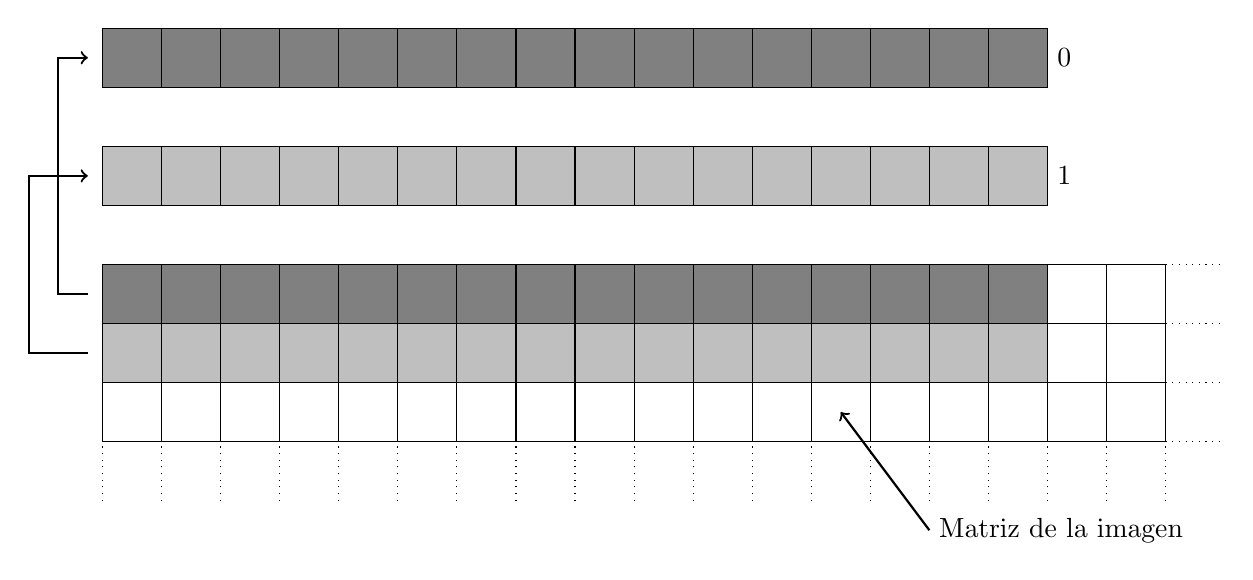
\begin{tikzpicture}[scale=0.75]
	        \foreach \x in {0, ..., 15}
	        {
	            % Registros
	            \filldraw[fill=gray]      (\x, 8) rectangle +(1, 1);
	            \filldraw[fill=lightgray] (\x, 6) rectangle +(1, 1);            

	            % Matriz
	            \filldraw[fill=gray]      (\x, 4) rectangle +(1, 1);
	            \filldraw[fill=lightgray] (\x, 3) rectangle +(1, 1);

	            % Líneas de proyección inferiores
	            \draw                     (\x, 2) rectangle +(1, 1);
	            \draw [dotted] (\x, 1) -- +(0, 1) ++(1, 0) -- +(0, 1);
	        }

	        \foreach \x in {16, 17}
	        {
	            % Matriz
	            \draw (\x, 4) rectangle +(1, 1);
	            \draw (\x, 3) rectangle +(1, 1);
	            \draw (\x, 2) rectangle +(1, 1);

	            % Líneas de proyección inferiores
	            \draw [dotted] (\x, 1) -- +(0, 1) ++(1, 0) -- +(0, 1);
	        }

	        \foreach \y in {2, ..., 5}
	        {
	            % Líneas de proyección laterales
	            \draw [dotted] (18, \y) -- +(1, 0);
	        }

	        % Etiquetas de los registros
	        \draw (16, 8.5) node[anchor=west]{\xmm{0}}
	             +( 0,  -2) node[anchor=west]{\xmm{1}};

	        % Etiqueta de la matriz
	        \draw (14, 0.5) node[anchor=west]{Matriz de la imagen};
	        \draw [->, thick] (14, 0.5) -- +(-1.5, 2);

	        % Flechas entre registros
	        \draw [->, thick] (-0.25, 3.5) -- ++(-1, 0)   -- ++(0, 3) -- +(1, 0);
	        \draw [->, thick] (-0.25, 4.5) -- ++(-0.5, 0) -- ++(0, 4) -- +(0.5, 0);

	    \end{tikzpicture}
		\caption{Obtención de los bloques a procesar en la iteración actual.}
		\label{bloques}
	\end{figure}

	\item El segundo paso consiste en desempaquetar los datos utilizando la instrucción PUNPCKHBW y PUNPCKLBW. Obteniendo de esta manera el valor de los pixeles en word's alojados en los registros $xmm0$,$xmm1$ los de la fila actual y en $xmm2$,$xmm3$ los de la siguiente fila.

	Es importante destacar en este paso, que la parte baja del registro $xmm0$ es desempaquetada en el mismo registro, miestras que la parte alta se desempaqueta guardando el resultado en el registro $xmm1$. lo mismo pasa con $xmm2$,$xmm3$, teniendo en cuenta que el valor del pixel es un Integer Unsigned, al desempaquetar completamos con $0$'s y seguimos teniendo la representación de el mismo número.

	\begin{figure}[H]
		\centering
		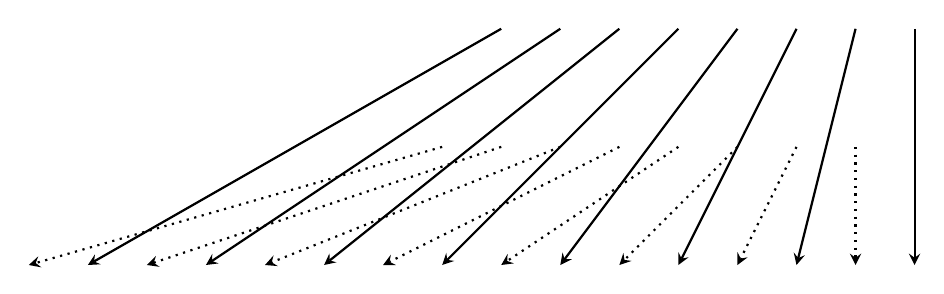
\begin{tikzpicture}[scale=0.75, >=stealth]
			\registroDieciseis{\xmm{0}}{0}{5}
				{A16}{A15}{A14}{A13}{A12}{A11}{A10}{A9}
				{A8} {A7} {A6} {A5} {A4} {A3} {A2} {A1}

			% Flechas A1, ... A8
			\foreach \x in {0, ..., 7}
			{
				\draw [->, thick] ({15.5 - \x}, 5) -- +({-\x}, -4);
			}

			% Flechas 0, ... 0
			\foreach \x in {0, ..., 7}
			{
				\draw [->, thick, dotted] ({14.5 - \x}, 3) -- +({-\x}, -2);
			}			

			\registroDieciseis{\texttt{XMMn}}{0}{3}
				{0}{0}{0}{0}{0}{0}{0}{0}
				{0}{0}{0}{0}{0}{0}{0}{0}				

			\registroDieciseis{\xmm{0}}{0}{0}
				{0}{A8}{0}{A7}{0}{A6}{0}{A5}
				{0}{A4}{0}{A3}{0}{A2}{0}{A1}
		\end{tikzpicture}
		\caption{Desempaquetado de los bytes a words.}
		\label{PUNPCK}
	\end{figure}

	\item El tercer paso del ciclo es sumar el valor de cada bloque de $2x2$. Para esto utilizamos $2$ instrucciones, PADDW y PHADDW. La primer instrucción es utilizada para sumar los valores de los pixeles de la fila actual con los valores de los pixeles correspondientes en la siguiente fila, obteniendo de esta manera en los registros $xmm0$ y $xmm1$ las sumas parciales de los bloques. O de otra forma; siendo $(i,j)$ y $(i+1,j)$ la posiciones de la imagen desde donde se obtienen los proximos $32$ pixeles a procesar, lo que obtenemos en el word más bajo de $xmm0$ es la suma del pixel $(i,j)$ con el pixel $(i+1,j)$ y asi hasta el word más alto de $xmm1$ donde tenemos la suma entre el pixel $(i,j+15)$ con el pixel $(i+1,j+15)$. Ver figura \ref{PHADDW}.

	La segunda instrucción (PHADDW) es utilizada para obtener la suma total de cada uno de los bloques. Tomando como ejemplo el bloque compuesto por los pixeles $(i,j)$,$(i,j+1)$,$(i+1,j)$ y $(i+1,j+1)$, ya tenemos las sumas parciales de los mismos en el registro $xmm0$. Más precisamente, tenemos en el word mas bajo del registro la suma de los pixeles $(i,j)$ y $(i+1,j)$ y el el siguiente word mas bajo la suma de los pixeles $(i,j+1)$ y $(i+1,j+1)$, por lo que al sumar estos dos word que se encuentran de manera consecutiva en el registro $xmm0$, lo que obtenemos es la suma total del bloque. 

	Dado que cada registro xmm tiene $8$ word y que para cada bloque las sumas parciales estan distribuidos en dos word consecutivos del mismo registro, la instrucción PHADD utilizando como operandos los registros $xmm0$ y $xmm1$ devuelven en el registro $xmm0$ efectivamente la suma total en cada word de cada uno de los $8$ bloques que se estan procesando en simultaneo.

	\begin{figure}[H]
		\centering
		\begin{tikzpicture}[scale=0.75]
			\draw (0,16) node[anchor=west]{Estado inicial de los registros:};

			\registroOcho{\xmm{0}}{-1}{14}{Y16}{Y15}{Y14}{Y13}{Y12}{Y11}{Y10}{Y9}

			\registroOcho{\xmm{1}}{1}{12}{Y8}{Y7}{Y6}{Y5}{Y4}{Y3}{Y2}{Y1}

			\registroOcho{\xmm{2}}{-1}{10}{X16}{X15}{X14}{X13}{X12}{X11}{X10}{X9}

			\registroOcho{\xmm{3}}{1}{8}{X8}{X7}{X6}{X5}{X4}{X3}{X2}{X1}

			\draw (0,7) node[anchor=west]
				{Luego de aplicar \asm{PADDW} \xmm{0}, \xmm{2} y
				                  \asm{PADDW} \xmm{1}, \xmm{3}:};

			\registroOcho{\xmm{0}}{-1}{5}
				{\small{X16+Y16}}{\small{X15+Y15}}{\small{X14+Y14}}{\small{X13+Y13}}
				{\small{X12+Y12}}{\small{X11+Y11}}{\small{X10+Y10}}{\small{X9+Y9}}

			\registroOcho{\xmm{1}}{1}{3}
				{\small{X8+Y8}}{\small{X7+Y7}}{\small{X6+Y6}}{\small{X5+Y5}}
				{\small{X4+Y4}}{\small{X3+Y3}}{\small{X2+Y2}}{\small{X1+Y1}}			

			\draw (0,2) node[anchor=west]
				{Luego de aplicar \asm{PHADDW} \xmm{0}, \xmm{1}:};

			\registroOcho{\xmm{0}}{0}{0}{}{}{}{}{}{}{}{}

			\draw (1,  1) node[anchor=north]{\scriptsize{X16+Y16+}}
			     +(0, -1) node[anchor=south]{\scriptsize{X15+Y15}}
                ++(2,  0) node[anchor=north]{\scriptsize{X14+Y14+}}
                 +(0, -1) node[anchor=south]{\scriptsize{X13+Y13}}
                ++(2,  0) node[anchor=north]{\scriptsize{X12+Y12+}}
                 +(0, -1) node[anchor=south]{\scriptsize{X11+Y11}}
                ++(2,  0) node[anchor=north]{\scriptsize{X10+Y10+}}
                 +(0, -1) node[anchor=south]{\scriptsize{X9+Y9}}
                ++(2,  0) node[anchor=north]{\scriptsize{X8+Y8+}}
                 +(0, -1) node[anchor=south]{\scriptsize{X7+Y7}}
                ++(2,  0) node[anchor=north]{\scriptsize{X6+Y6+}}
                 +(0, -1) node[anchor=south]{\scriptsize{X5+Y5}}
                ++(2,  0) node[anchor=north]{\scriptsize{X4+Y4+}}
                 +(0, -1) node[anchor=south]{\scriptsize{X3+Y3}}
                ++(2,  0) node[anchor=north]{\scriptsize{X2+Y2+}}
                 +(0, -1) node[anchor=south]{\scriptsize{X1+Y1}};

            % Flecha izquierda
            \draw [->, thick] (-2.5, 14.5) -- ++(-0.5, 0) -- ++(0, -9) -- +(0.5, 0);
            \draw [thick] (-3, 10.5) -- +(0.5, 0);

            % Flecha derecha
            \draw [->, thick] (17.5, 12.5) -- ++(0.5, 0) -- ++(0, -9) -- +(-0.5, 0);
            \draw [thick] (18, 8.5) -- +(-0.5, 0);
		\end{tikzpicture}

		\caption{suma total de los bloques que se estan procesando.}
		\label{PHADDW}
	\end{figure}

	\item El cuarto paso consiste en reemplazar cada bolque de $2x2$ por el bloque que le corresponda dependiendo de el valor obtenido en la suma total del mismo.

	Para esto utilizamos los registros $xmm12$ al $xmm15$, en los cuales estan guardados en paquet word los valores $205$,$410$,$615$ y $820$.

	Mirando como son los bloques predefinidos en el enunciado, y teniendo en cuenta que el valor $255$ que reprecenta al blanco en un byte es $0xff$ y el del negro es $0x0$, armamos dos mascaras con los valores

	$0x00ff00ff00ff00ff00ff00ff00ff00ff$ y $0xff00ff00ff00ff00ff00ff00ff00ff00$. 

	Estas mascaras dejan los valores ya seteados en bytes, por lo que luego no hay que empaquetarlos.
	Para entender bien la idea observemos primero lo siguiente:

	Cada pixel de la imagen ocupa un byte, pero como arrancamos de la posición $0$ y siempre nos movemos una cantidad par de posiciones en cada iteración (en particular nos movemos de a $16$ pixeles), sabemos que en los registros donde guardaremos el resultado para mandar al destino, cada par contiguo de pixeles pertenese a un mismo bloque de $2x2$, dado que la suma total de cada bloque también está guardada en word's, y que dos pixeles contiguos ocupan un word, podemos ver que la suma de un bloque abarca a todos los pixeles del mismo.

	Luego, obtenemos la mascara resultante de comparar la suma total de los boques que se estan procesando con los valores $205$,$410$,$615$ y $820$. Esta mascara está en word's empaquetados, en los cuales hay unos o ceros dependiendo de si el word pertenece a un bloque cuya suma es mayor o menor que los valores con los que es comparado. 

	Sabiendo que para todo bloque mayor a $205$ el primer pixel de la primer fila debe ser blanco. a la mascara de comparaciones le aplicamos la mascara con los valores  

	$0xff00ff00ff00ff00ff00ff00ff00ff00$ y lo que obtuvimos fue que para aquellos boques mayores a $205$ los bytes de posiciones pares tienen unos, mientras que los impares tienen ceros. Como vimos recién, el hecho que el byte tenga unos es lo mismo a que tenga un $255$ por lo que de esta manera ya tenemos en la mascara resultante los valores deseados para las posiciones pares de la primer fila y ceros en las posiciones impares.

	Esto mismo es realizado para los valores $410$,$615$ y $801$ obteniendo en $4$ registros $xmm$ los valores de cada pixel procesado, luego para unir estos valores, se hace un POR entre los dos registros pertenecientes a la primer fila y otro POR entre los dos registros pertenecientes a la segunda fila y asi obtenemos el resultado ya listo para mandar a memoria.

	La instrucción utilizada para estas comparaciones es PCMPGTW.

	\item El ultimo paso consiste en guardar en la memoria correspondiente los pixeles ya procesados.

\end{itemize}

\subsubsection{Comparación con el lenguaje C}
Mirando el pseudocodigo del algoritmo en C se puede ver que la principal diferencia es que mientras que en un ciclo del codigo en C se procesa un solo bloque, en assembler estamos procesando 8. Pero ademas de esto, para obtener los pixeles de un bloque en C tenemos que hacer 4 llamados a memoria mientras que en assembler para obtener los 8 bloques hacemos 2 llamados en memoria.	Esto mismo se repite a la hora de guardar los datos en la imagen de destino.

Por otro lado teniendo en cuenta ciertas propiedades, como el hecho de que un byte con todos unos es un byte con un $255$ en Unsigned Integer, en la version assembler sabemos que al crear la mascara ya tenemos colocado el valor deseado. El compilador no utiliza tales propiedades como tampoco utiliza instrucciones SIMD. Es por esto que ademas de utilizar instrucciones de comparación agrega instrucciónes para insertar los valores deseados, generando mas lentitud en el algoritmo. 

Si nos ponemos a ver con un poco mas de detalles, para realizar la suma del bloque que se esta procesando, en C se utilizan cuatro repeticiones de la instrucción ADD por cada bloque, por lo cual se realizan $32$ ADD para obtener la suma de 8 bloques, mientras que al utilizar SIMD, con 2 instrucciones PADDW y una instruccion PHADDW obtenemos las mismas sumas.

\subsubsection{Rendimiento}

Observamos las siguientes cantidades de ciclos y ticks de reloj al realizar 100 iteraciones de ambas implementaciones con una imagen cuadrada de lado 512.

\begin{center}
    \begin{tabular}{|l|l|l|l|}
        \hline
        Medición & Implementación C & Implementación assembler & Relación \\
        \hline
        Ticks    & 785867600      & 70172072               & $8.92\%$ \\
        Ciclos   & 7858676        & 701721                 & $8.92\%$ \\
        \hline
    \end{tabular}
\end{center}